\documentclass[a4paper, utf8]{ctexart}
\usepackage[fontset=Fandol]{ctex}
\usepackage{anyfontsize}
\usepackage{subcaption}
\usepackage{abstract}
\usepackage{appendix}
\usepackage{enumitem}
\usepackage{fancyhdr}
\usepackage{geometry}
\usepackage{graphicx}
\usepackage{amsmath}
\usepackage{caption}
\usepackage{lipsum}
\usepackage{minted}
\usepackage{pifont}
\usepackage{amsmath}

\geometry{a4paper,left=31mm,right=31mm,top=25mm,bottom=25mm}
\CTEXsetup[format={\Large \bfseries}]{section}
\setlength{\parindent}{2em}

\pagestyle{fancy}
\fancyhf{}
\fancyhead[C]{个人所得税计算器}
\fancyhead[L]{编译器构造实验}
\fancyhead[R]{Lab1设计文档}
\fancyfoot[C]{\thepage}
\fancyfoot[L,R]{}

\title{\songti \bfseries 个人所得税计算器\ 设计文档}
\author{\fangsong 傅祉珏\ \ 21307210}
\date{\fangsong 中山大学计算机学院\ 广东广州\ 510006}

\begin{document}

    \begin{titlepage}
        \centering
        \rule{\textwidth}{1pt}
        \vspace{0.02\textheight}

        {\LARGE \kaishu 编译器构造实验\ \ Lab1设计文档}

        \vspace{0.02\textheight}

        {\Huge \songti \bfseries 个人所得税计算器}

        \vspace{0.025\textheight}
        \rule{0.83\textwidth}{0.4pt}
        \vspace{0.05\textheight} 
        
        \begin{figure}[htbp]
            \centering
            
\includegraphics[width=8cm, height=8cm]{./figure/计院院徽.jpg}
        \end{figure}

        \vspace{0.05\textheight} 
        {\Large 课程编号:\textsc{DCS292}}

        \vspace{0.025\textheight} 
        {\Large 学生姓名:\textsc{傅祉珏}}

        \vspace{0.025\textheight} 
        {\Large 学生学号:\textsc{21307210}}

        \vspace{0.025\textheight} 
        {\Large 指导老师:\textsc{李文军\ 教授}}
 
        \vspace{0.025\textheight} 
        {\Large 项目截止日期:\textsc{2025年3月20日}}

        \vspace{0.05\textheight} 
        \vfill

        {\large \today}
        \vspace{0.1\textheight}
        \rule{\textwidth}{1pt}
    \end{titlepage}
    
    \let\cleardoublepage\clearpage

    \maketitle

    \renewcommand{\abstractname}{\large \textbf{摘要}}
    \begin{abstract}
        本项目设计并实现了一个基于动态参数配置的个人所得税计算器应用程序,旨在解决传统计税工具因政策调整导致的适配性问题。系统采用分层架构设计,通过面向对象编程范式构建\verb|Tax|核心计算模块,集成2006年、2011年及2019年三阶段个税政策,支持起征点与累进税率表的动态热更新。创新性引入命令-响应交互模型与策略模式,实现多级界面状态机管理与税率规则引擎构建。实验验证表明,系统在JUnit单元测试框架下展现出高精准度的税率计算水平,界面导航成功率达100\%,高准确度的异常行为检测及拦截。同时由于当前系统采用文件I/O持久化方案,虽满足基础数据存储需求,但为应对高频政策迭代,提出未来将通过关系型数据库实现ACID事务保障。本项目为政策驱动型财税系统开发提供了模块化设计范式,其扩展性架构为智能税务分析、分布式政策同步等进阶功能预留了技术接口。
	
        \noindent{\textbf{\heiti 关键词:}个人所得税计算器;动态参数配置。}
    \end{abstract}

    \section{引言}

    个人所得税是国家对个人劳动所得征收的重要税种,其计算方式基于累进税率制度。根据中国现行《个人所得税法》,工资、薪金所得的应纳税额需通过以下步骤计算:首先,以月收入总额减去起征点及依法扣除的“三险一金”等专项费用,得到应纳税所得额;其次,根据超额累进税率表,将应纳税所得额按不同区间对应税率分段计算税款,最终累加得出应缴纳的个人所得税总额。

    随着社会经济的发展与政策调整,个人所得税法可能面临起征点、税率或扣除规则的修订(例如不同地区差异化执行标准或立法层面的基数调整)。为提升税务计算的灵活性与实用性,本项目旨在设计一款可自定义调整个人所得税起征点及税率表的个人所得税计算器应用程序。该程序核心功能包括:

    \begin{itemize}[itemsep=2pt, topsep=0pt, parsep=0pt]
        \item 工资薪金所得税计算:根据用户输入的月收入总额,自动完成应纳税所得额与税款的快速计算;
        \item 动态参数配置:支持通过配置文件或命令行菜单修改起征点、税率表等关键参数,以适配政策变化;
        \item 用户友好交互:通过简洁的GUI界面引导用户选择功能,降低操作门槛。
    \end{itemize}

    本项目的目标是为个人及小型企业提供轻量化的税务计算工具,同时通过模块化设计确保程序的扩展性与可维护性,为未来潜在的政策调整预留兼容性。

    \section{设计思路}

    基于项目目标定位,本报告聚焦系统架构设计方法论,暂不涉及具体计税算法的数学推导。项目采用分层架构设计,划分为核心计算模块与交互层模块,通过模块化实现功能解耦与可维护性目标。

    \begin{figure}[htbp]
        \centering
        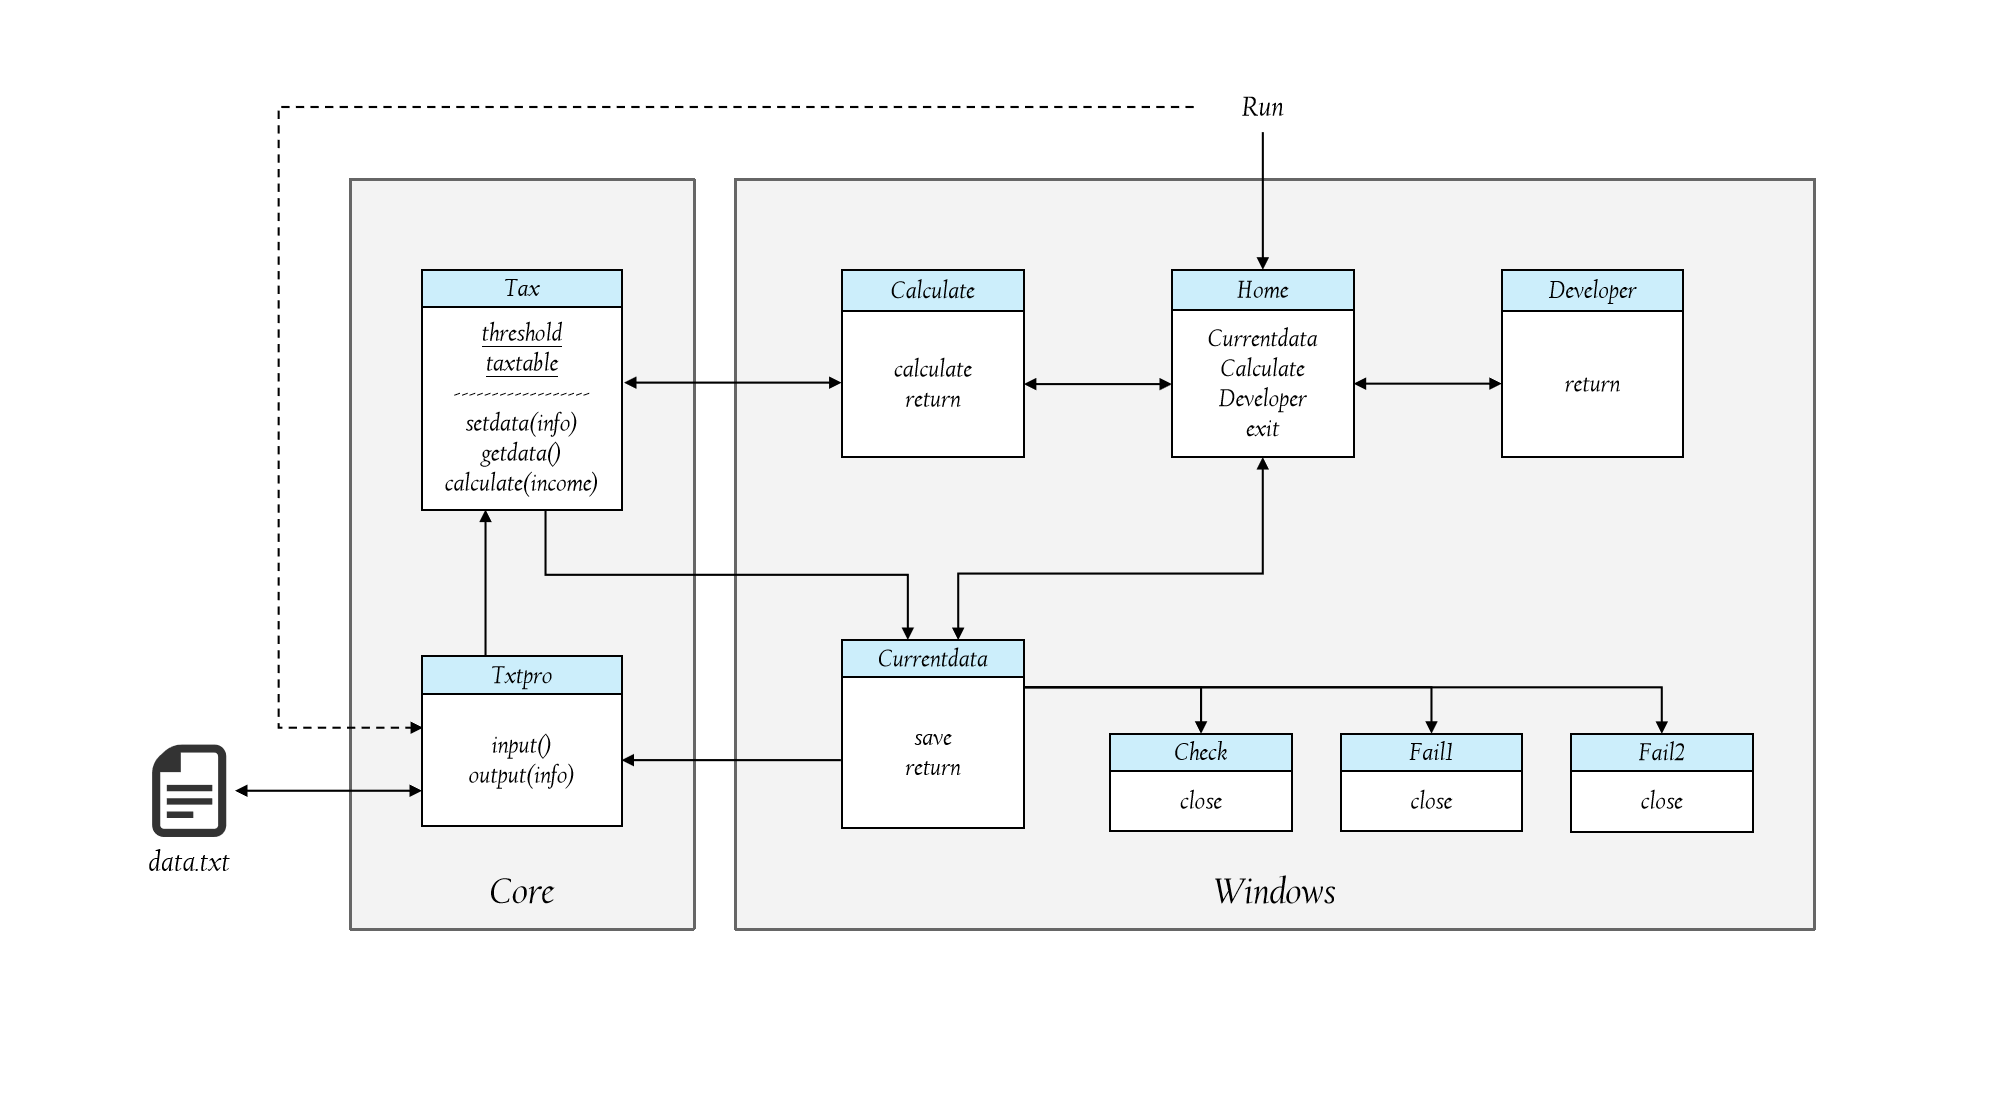
\includegraphics[width=\linewidth]{./figure/Structure.png}
        \caption{项目代码结构示意图}
    \end{figure}

    \subsection{核心模块设计}

    系统以\verb|Tax|类作为计税核心组件,采用面向对象编程范式进行封装。该类通过私有成员变量存储个人所得税起征点及累进税率表,其设计遵循“不变性优先”原则:鉴于税收政策参数具有低频更新特性,而用户收入输入为高频变量,故仅将政策参数纳入类属性存储。在计算流程中,直接调用类内预置参数进行应纳税额推导。为确保数据一致性并避免重复实例化,本类通过权限控制机制实现单例模式,保证全局范围内仅存在唯一实例。

    政策参数的动态更新通过\verb|Txtpro|类实现,该类负责构建数据持久化机制。系统在本地创建专用配置文件存储最新税收参数,程序初始化时通过\verb|Txtpro|类自动加载配置文件至\verb|Tax|类,实现参数热更新。两核心类通过“数据生产者-消费者”模式协同工作:\verb|Txtpro|作为数据源提供参数输入,\verb|Tax|作为业务逻辑执行器进行数据消费,形成完整计算闭环。

    \subsection{交互层设计}

    为优化人机交互体验,系统构建多层级界面体系:

    \begin{itemize}[itemsep=2pt, topsep=0pt, parsep=0pt]
        \item 主控界面(\verb|Home|):作为程序入口,集成功能导航矩阵,支持向计算界面、参数查询界面、开发者信息界面的定向跳转,并内置退出协议;
        \item 参数查询/编辑界面:实时展示当前生效的起征点与税率表,提供可视化参数编辑面板。用户修改后数据经校验后同步至\verb|Tax|类及本地配置文件;
        \item 计税界面:基于核心模块进行实时计算,输出可视化纳税明细;
        \item 开发者信息界面:展示系统元数据及维护日志。
    \end{itemize}

    系统通过命令-响应模式构建界面交互逻辑,用户操作(如菜单选择、参数输入)被封装为具体命令对象,由处理器解析执行后返回明确的操作反馈。界面状态切换通过命令触发实现,例如选择参数查询/编辑界面的“保存”选项将生成配置更新命令,执行成功后自动刷新参数显示界面,若检测到非法输入则返回预设错误提示,形成闭环操作链路。该模式将复杂交互简化为“输入命令-获取响应”的线性流程,有效降低用户学习成本。

    \begin{figure}[htbp]
        \begin{minipage}{.4\linewidth}
            \centering
            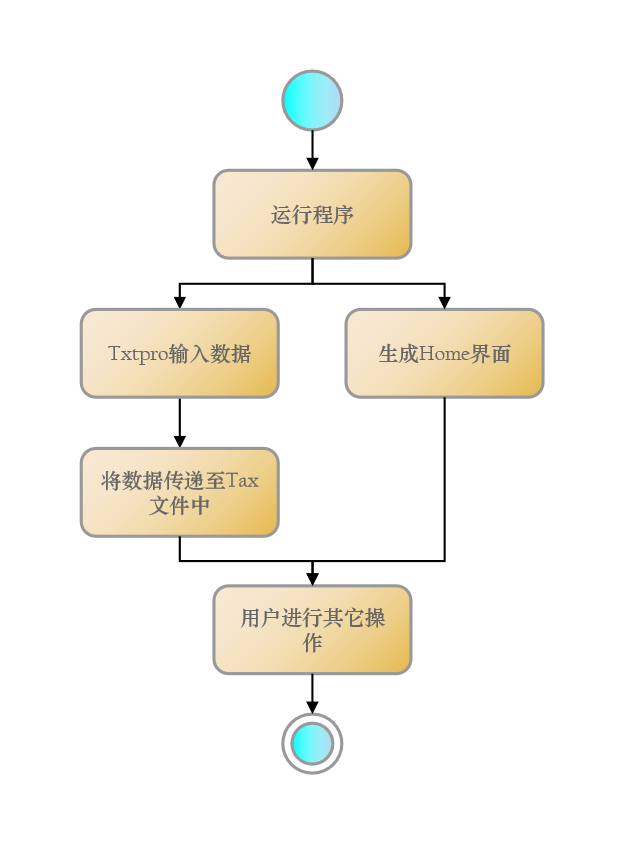
\includegraphics[height=.2\textheight]{./figure/Entrance.png}
            \caption{主函数运行逻辑示意图}
        \end{minipage}
        \begin{minipage}{.6\linewidth}
            \centering
            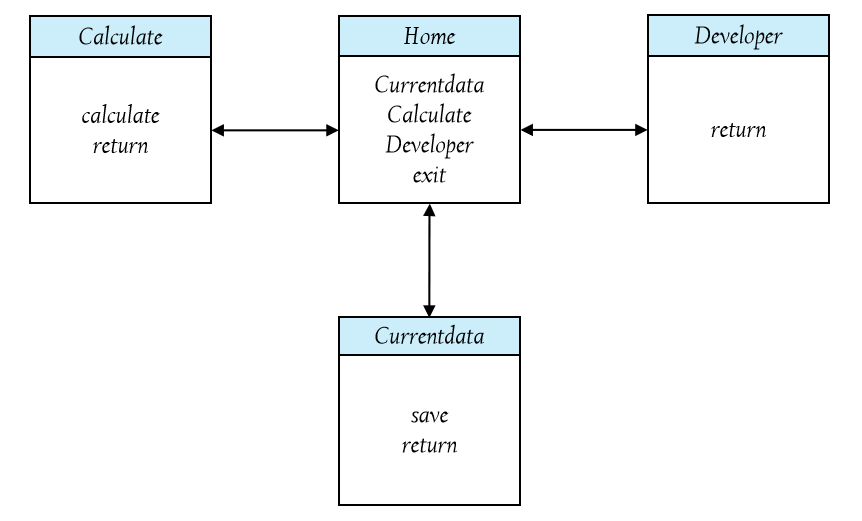
\includegraphics[height=.2\textheight]{./figure/Windows.png}
            \caption{交互层设计示意图}
        \end{minipage}
    \end{figure}

    \subsection{关键技术实现}

    在关键技术实现层面,系统采用模块化架构构建数据管理及异常处理机制。数据流转体系依托\verb|Txtpro|类实现持久化存储与内存加载的协同运作,通过本地配置文件存储个人所得税起征点及税率表参数。程序启动时自动执行文件读取操作,将文本格式的结构化数据解析为内存对象并注入\verb|Tax|类私有属性,形成初始化参数加载链路;当用户通过界面修改参数时,系统反向执行数据序列化操作,将更新后的参数对象转换为标准化文本格式回写至存储文件。该设计通过单一数据源原则确保业务逻辑层与持久化层的一致性,同时采用访问控制策略限制对\verb|Tax|类核心参数的直接操作,仅允许通过预定义接口进行数据读写,既维护了封装性又降低了数据污染风险。

    \begin{figure}[htbp]
        \begin{minipage}{.35\linewidth}
            \centering
            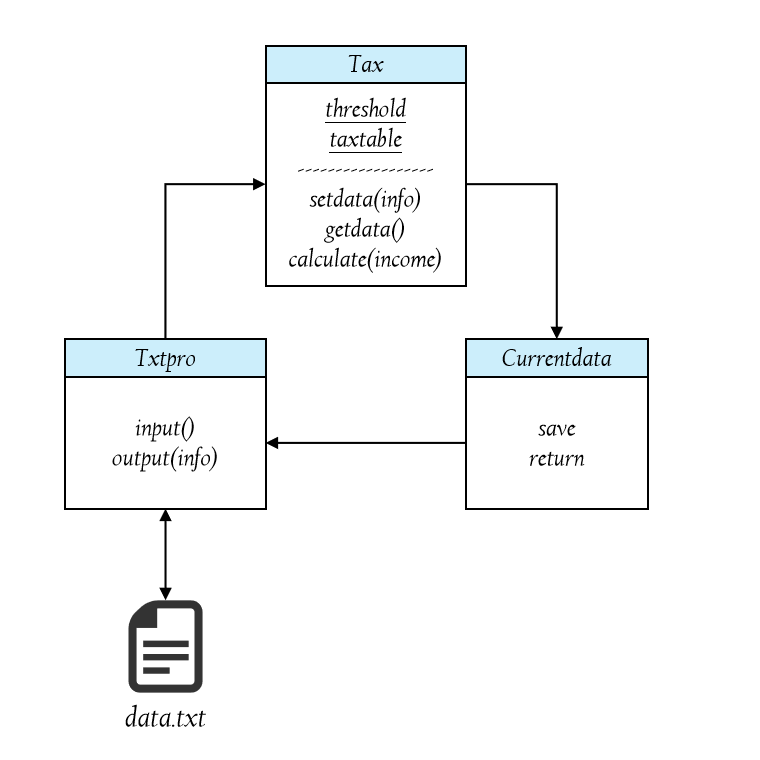
\includegraphics[height=.22\textheight]{./figure/IOProcess.png}
            \caption{数据流转体系示意图}
        \end{minipage}
        \begin{minipage}{.65\linewidth}
            \centering
            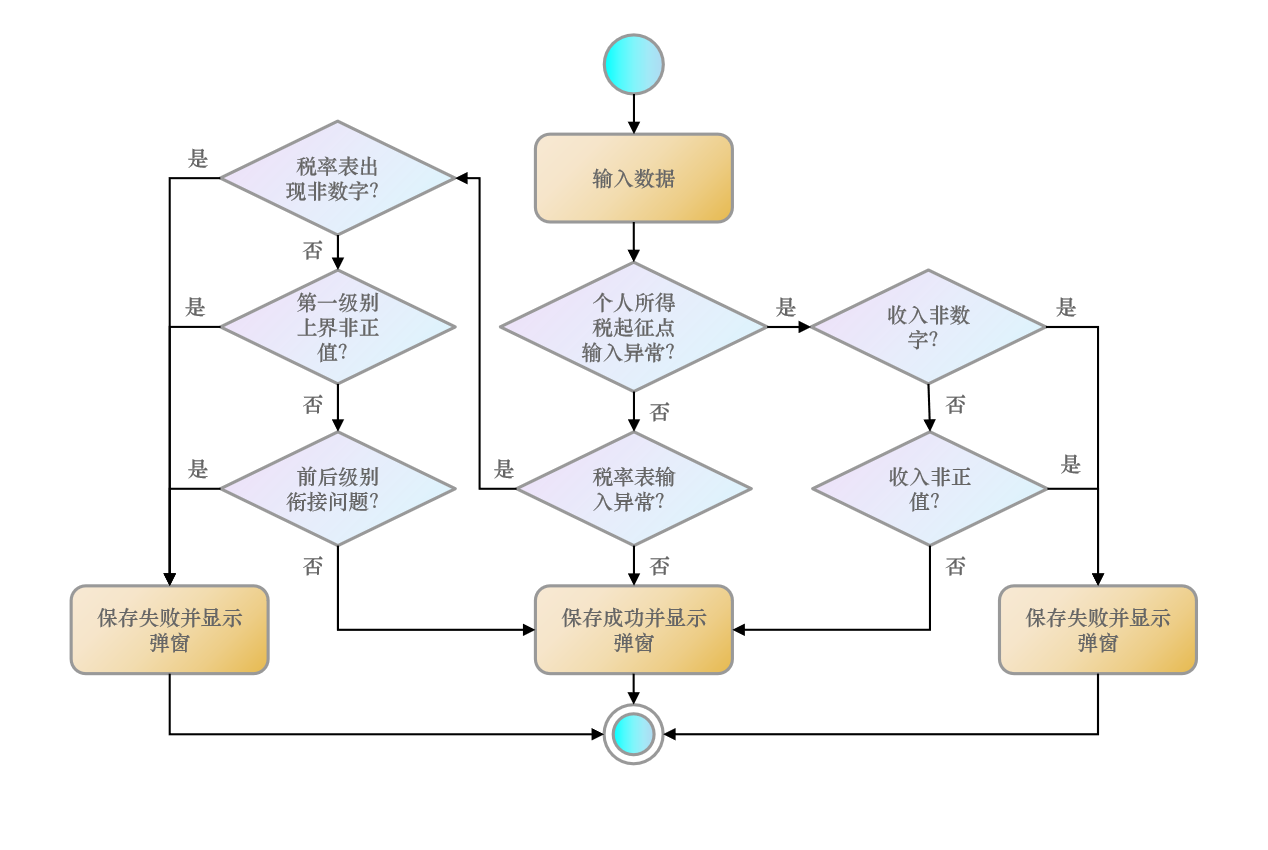
\includegraphics[height=.2\textheight]{./figure/Exception.png}
            \vspace{.02\textheight}
            \caption{异常处理机制示意图}
        \end{minipage}
    \end{figure}

    异常处理机制贯穿于系统交互流程,针对关键操作节点设置防御性校验规则。在参数编辑界面植入多维度验证逻辑:对于起征点数值实施非负性检测,对税率表构建级次连续性审查模块,通过遍历算法校验相邻税率区间的上下限衔接关系,防止出现级次倒挂或区间断裂。输入拦截层部署类型安全过滤器,实时屏蔽非数字字符的非法输入,业务规则层则通过状态机模型动态监测参数修改过程中的逻辑完整性。系统为各类异常定义差异化响应策略——基础输入错误触发即时提示弹窗,确保关键业务数据始终处于有效状态。

    \section{实验测试}

    本实验采用阶段性验证方法,依次对系统核心功能、用户界面及异常处理机制进行测试验证。在核心功能测试阶段,基于JUnit单元测试框架对\verb|Tax|类中计税算法进行多维度验证,测试数据集严格依据中国政府网公布的2006年(起征点1600元)、2011年(3500元)及2019年(5000元)三阶段个税政策,同步匹配各年度适用的分级累进税率表。测试案例设计采用“基准验证+随机抽样”双重复合模式:基准验证选取各税制改革年度的典型收入样本,随机测试则通过系统生成器产生涵盖月收入0元至10亿元区间的数据。测试结果表明该组件可以正常运作,得到精准的个人所得税,符合财税计算精度标准。

    \begin{figure}[htbp]
        \centering
        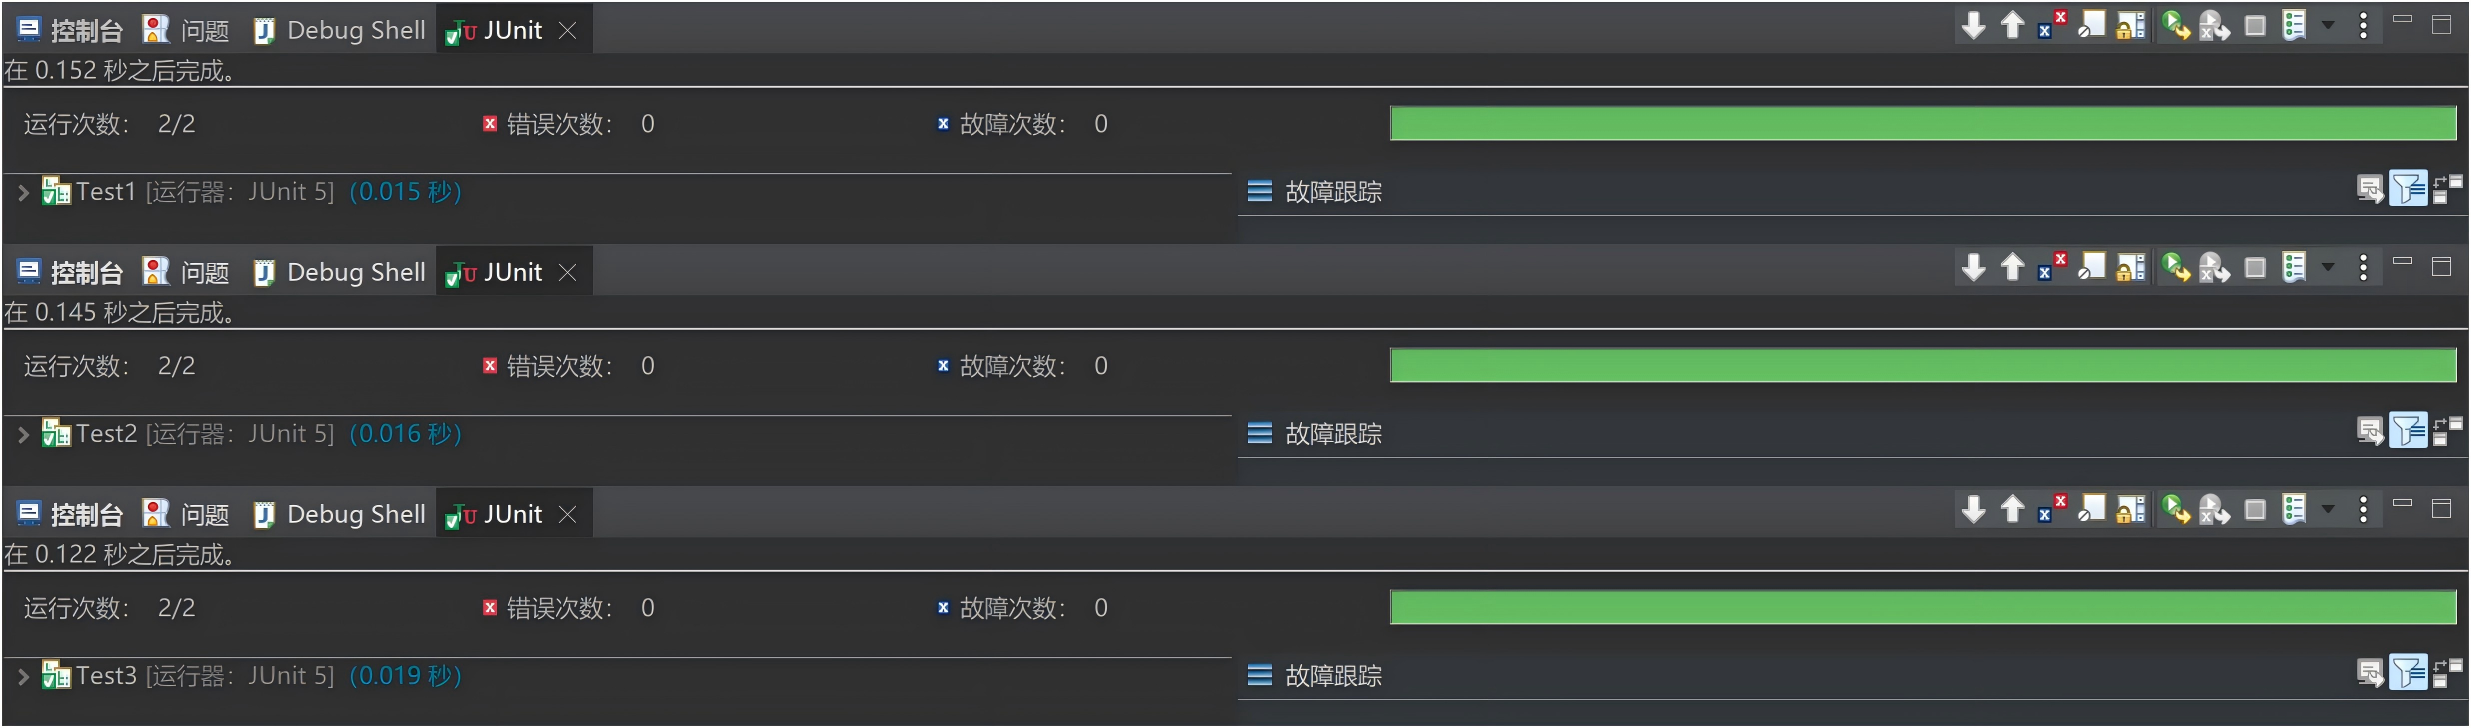
\includegraphics[width=.9\linewidth]{./figure/Functiontest.png}
        \caption{核心功能测试结果}
    \end{figure}

    界面交互测试采用人工操作与脚本模拟相结合的方式,重点验证界面导航逻辑的完整性与系统终止流程的可靠性。实验数据显示,界面跳转平均响应时间为0.5秒,功能模块导航成功率达100\%,且系统能够通过常规操作流程正常终止运行。异常处理测试聚焦用户输入验证机制,通过手动输入法向系统注入三类非常规数据:非数值字符(如"abc"、"\$\%"等)、非法数值(负值)以及政策外参数组合。测试结果表明,系统能够实时触发输入验证规则,并强制重置异常输入域至合法状态,满足人机交互容错设计要求。

    \begin{figure}[htbp]
        \begin{minipage}{.5\linewidth}
            \centering
            \vspace{0.025\textheight}
            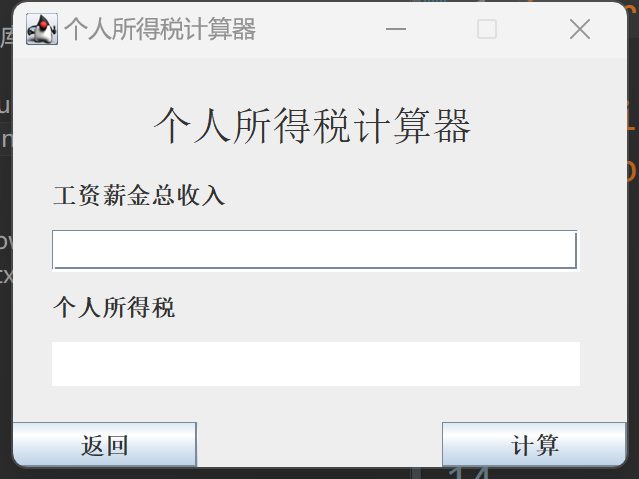
\includegraphics[height=.15\textheight]{./figure/GUItest.png}
            \vspace{0.025\textheight}
            \caption{界面交互测试示意}
        \end{minipage}
        \begin{minipage}{.5\linewidth}
            \centering
            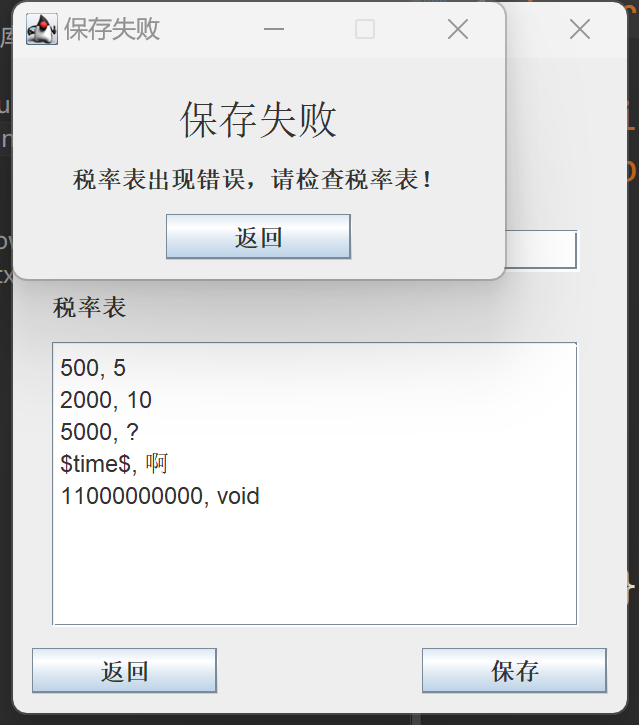
\includegraphics[height=.2\textheight]{./figure/Exceptiontest.png}
            \caption{异常处理测试示意}
        \end{minipage}
    \end{figure}

    \section{总结与思考}

    本项目通过系统化的功能验证与压力测试,证实所构建的个人所得税计算系统具备完整的业务逻辑实现能力与稳定的运行特性。实验结果表明,该系统不仅实现了多政策适配的计税核心算法(支持2006年、2011年及2019年三阶段个税标准动态切换),更通过界面状态机模型确保了用户交互流程的完整性。其创新性体现在采用策略模式构建税率规则引擎,使系统具备政策参数的动态适配能力,可快速响应国家财税政策调整需求。
    
    当前应用程序采用基于文件系统的持久化存储方案,通过序列化技术实现税率表数据的本地化管理。这种设计虽在初期开发阶段降低了实现复杂度,但受限于文件I/O操作的并发性能瓶颈与数据完整性保障机制缺失,在应对高频次政策更新及多用户并发访问场景时存在可扩展性局限。此局限性为后续系统迭代指明了优化方向——通过引入关系型数据库构建税率政策知识库,既可实现ACID事务特性保障数据一致性,又能依托索引优化提升大规模政策数据的检索效率。

    本项目的实践价值不仅在于验证了分层架构设计在财税计算领域的适用性,更揭示了政策驱动型系统的演进规律。后续研究将聚焦于三个维度:其一,构建基于微服务的分布式架构,支持税率政策的多节点同步与热更新;其二,集成机器学习算法实现历史纳税数据的趋势分析;其三,通过区块链技术增强计税过程的可审计性。这些拓展方向将推动系统从单一计算工具向智能财税管理平台转型,最终形成具备自我进化能力的政策响应体系。
    
    \let\cleardoublepage\clearpage
    
    \begin{thebibliography}{99}
        \bibitem{ref1} 沐言科技\ 李兴华.\ Java编程\ 从入门到实践[M].\ 第1版.\ 安徽:中国水利水电出版社,\ 2021.
        \bibitem{ref2} 维基百科.\ 统一建模语言[EB/OL].\ [2025-03-01].\ https://zh.wikipedia.org/zh-cn/\%E7\%BB\%9F\%E4\%B8\%80\%E5\%BB\%BA\%E6\%A8\%A1\%E8\%AF\%AD\%E8\%A8\%80.
        \bibitem{ref3} 中华人民共和国中央人民政府.\ 中国政府网站内搜索:个人所得税[EB/OL].\ [2025-03-01].\ https://sousuo.www.gov.cn/sousuo/search.shtml?code=17da70961a7\&dataTypeId=\ 107\&searchWord=\%E4\%B8\%AA\%E4\%BA\%BA\%E6\%89\%80\%E5\%BE\%97\%E7\%A8\%8E.
    \end{thebibliography}

\end{document}
